\documentclass{beamer}

%Russian-specific packages
%--------------------------------------
\usepackage[T2A]{fontenc}
\usepackage[utf8]{inputenc}
\usepackage[english,main=russian]{babel}
%--------------------------------------

\usepackage{graphicx}
\usepackage{amssymb,amsmath}
\usepackage{pgfplots, pgfplotstable}
\pgfplotsset{compat=newest}
\pgfplotstableread[col sep=comma]{../data/heuristic-00.csv}\heuristicno
\pgfplotstableread[col sep=comma]{../data/heuristic-15.csv}\heuristicsome
\pgfplotstableread[col sep=comma]{../data/random.csv}\random
\makeatletter
\pgfplotsset{
    /pgfplots/flexible xticklabels from table/.code n args={3}{%
        \pgfplotstableread[#3]{#1}\coordinate@table
        \pgfplotstablegetcolumn{#2}\of{\coordinate@table}\to\pgfplots@xticklabels
        \let\pgfplots@xticklabel=\pgfplots@user@ticklabel@list@x
    }
}
\makeatother

\graphicspath{{logo/}{pics/}}
\beamertemplatenavigationsymbolsempty{}
\setbeamertemplate{footline}[frame number]
\setbeamerfont{footline}{size={\fontsize{10}{12}}}

\title{Оптимизация функции, задаваемой регрессионным лесом}
\author{Влад Ягламунов}
\date{}

\begin{document}

\begin{frame}
\maketitle
{\small 
    \textbf{Формальный научный руководитель:}\par Фильченков Андрей Александрович\par
    \textbf{Фактический научный руководитель:}\par Шаламов Вячеслав Владимирович
}
\end{frame}

\begin{frame} \frametitle{Задача}
    \begin{itemize}
        \item \textbf{Дано:} Обученный регрессионный лес
        \item \textbf{Найти:} Области, где лес возвращает минимальное и максимальное значение
    \end{itemize}
\end{frame}

\begin{frame} \frametitle{Применение}
    Random Forest:
    \begin{itemize}
        \item Суррогатные функции для оптимизации
        \item Хорошо обновляется при добавлении информации \pause{}
        \item Последовательная оптимизация основанная на модели Sequential Model-Based Optimization (SMBO)
        \item Sequential Model-based Algorithm configuration (SMAC)
    \end{itemize}
    \vfill
    \pause{}
    Сейчас используется перебор случайного набора точек.
    \vfill
\end{frame}

\begin{frame} \frametitle{Random Forest}
    \begin{columns}
        \column{.6\textwidth}
            \begin{itemize}
                \item Ансамбль деревьев принятия решения
                \item Каждое дерево обучено на случном подмножестве
                \item Результат: среднее всех деревьев 
                \item Пространство разбивается на прямоугольники по ''трешхолдам'' вершин
            \end{itemize}
        \column{.4\textwidth}
        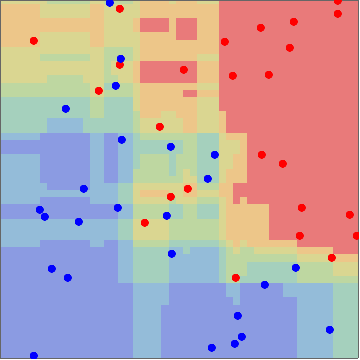
\includegraphics[width=\textwidth]{random_forest.png}
    \end{columns}
\end{frame}

\begin{frame} \frametitle{Эвристический алгоритм}
    \begin{columns}
        \column{.5\textwidth}
            \begin{itemize}
                \item Перебор по всем поддеревьям
                \item Для вершины храним минимум и максимум в поддереве
                \item Поддерживаем, что все поддеревья пересекаются
            \end{itemize}
        \column{.5\textwidth}
            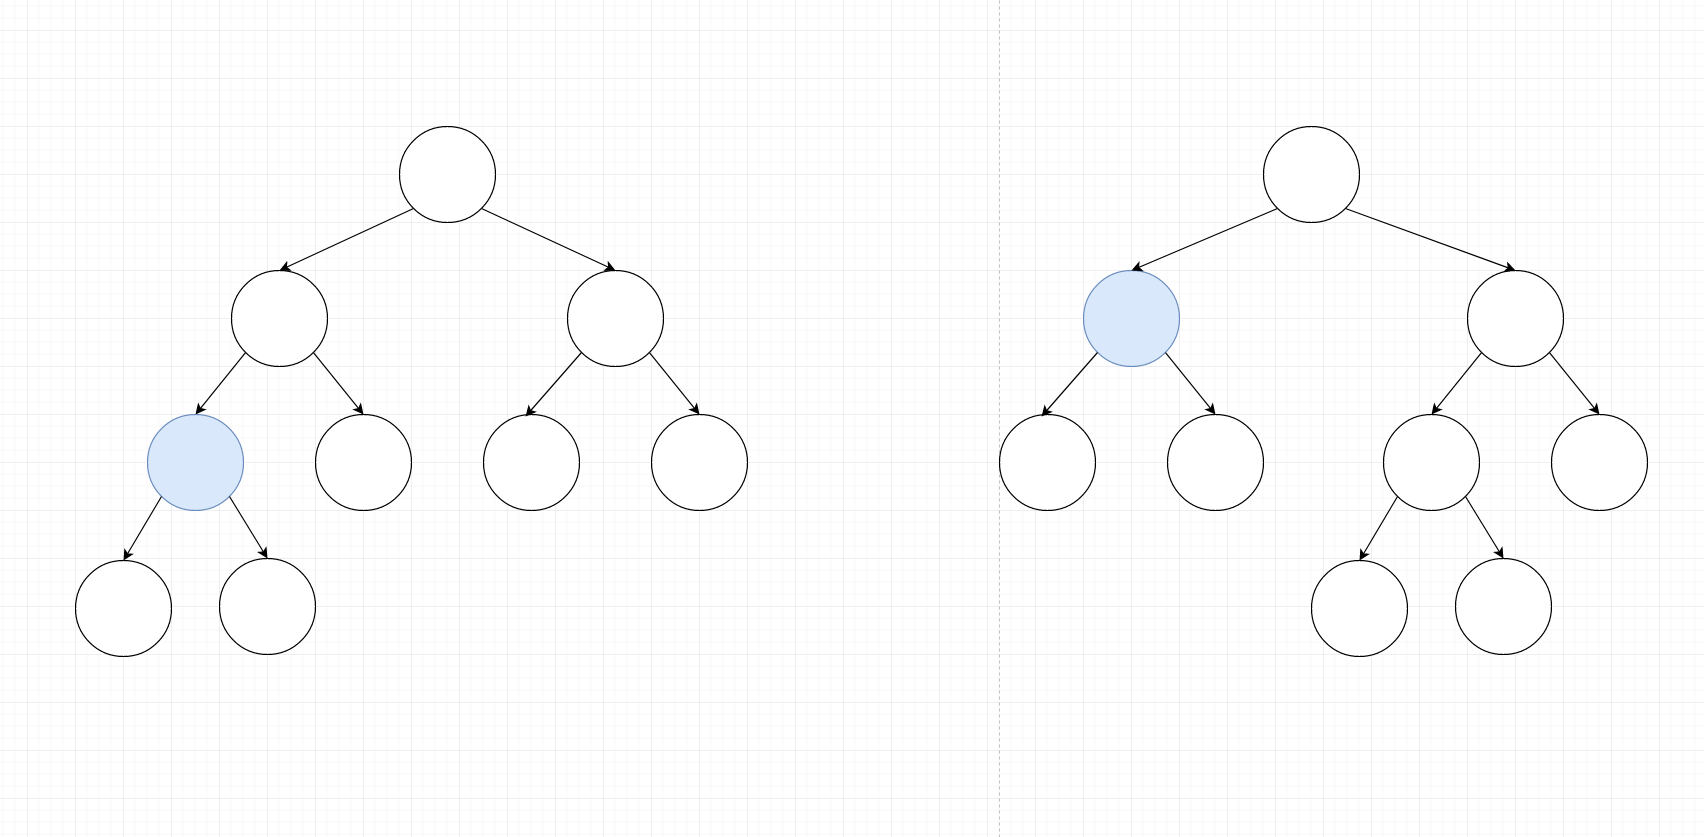
\includegraphics[width=\textwidth]{tree.png}
    \end{columns}
\end{frame}

\begin{frame} \frametitle{Эвристический алгоритм}

    \begin{columns}
        \column{.75\textwidth}
            На каждом шаге рассматриваем n-мерный прямоугольник области

            Шаг: разбиение по трешхолду вершины
        \column{.25\textwidth}
            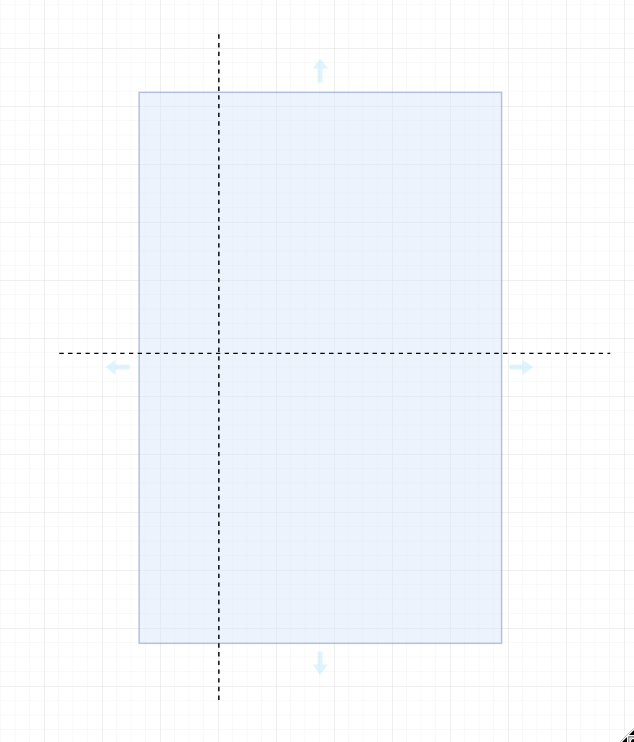
\includegraphics[width=\textwidth]{split.png}
    \end{columns}
    \vfill
    \pause{}
    Эвристика:
    \[
        i = \arg \max_{v \in trees}(|value[v.left] - value[v.right]|)
    \]
\end{frame}

\begin{frame} \frametitle{Эвристический алгоритм (Оптимизация 1)}
    Необязательно искать точное решение.

    \vspace{50px}
    Не будем перебирать поддерево, если в лучшем случае это не улучшит ответ хотя бы на $\alpha$

    \[
        value[v] < \alpha current
    \]

    Гарантирует точность $>\alpha$
\end{frame}

\begin{frame} \frametitle{Эвристический алгоритм (Оптимизация 2)}
    Максимум в поддереве может не пересекаться с текущей областью

    \begin{columns}
        \column{.5\textwidth}
            \begin{itemize}
                \item Отсортированный список всех его листьев
                \item На каждом шаге в таком списке мы движемся только вперёд
            \end{itemize}
        \column{.5\textwidth}
            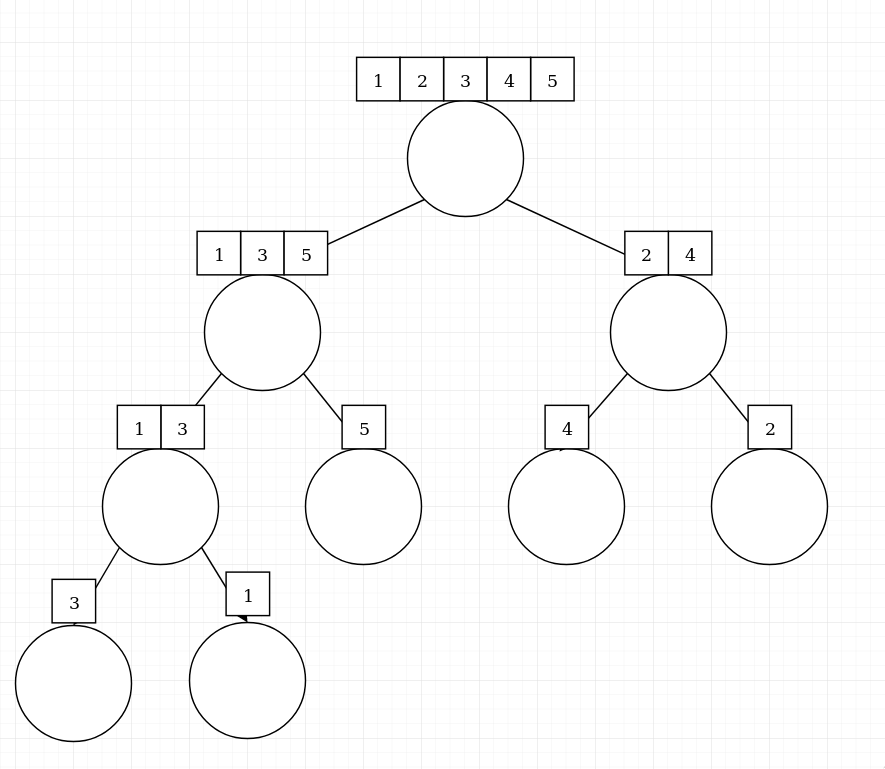
\includegraphics[width=1.1\textwidth]{merge.png}
    \end{columns}
\end{frame}

\begin{frame} \frametitle{Алгоритм имитации отжига}
    \begin{center}
    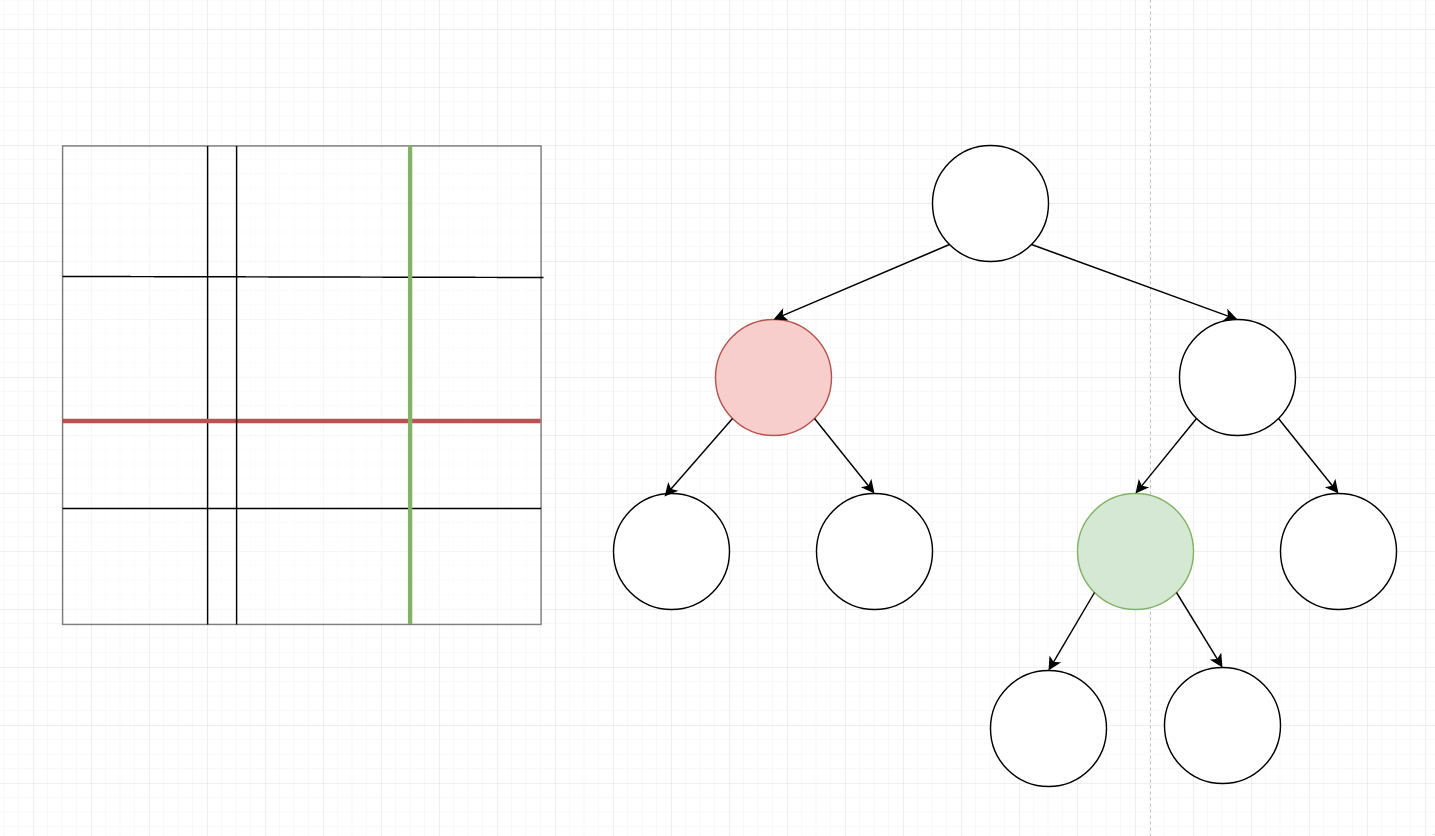
\includegraphics[width=0.8\textwidth]{gena.png}
    \end{center}
    \begin{itemize}
        \item Разбиваем пространство по всем трешхолдам
        \item Случайные мутации по переходе в соседнюю клетку
        \item Достаточно пересчитать только одно дерево
    \end{itemize}
\end{frame}

\begin{frame} \frametitle{Алгоритм имитации отжига}
\begin{columns}
    \column{.5\textwidth}
    Если значение ухудшилось, то переходим с вероятностью уменьшающейся от температуры (номера итерации)
    \[
    p=\alpha + (1 - \alpha) \frac{i}{N}
    \]
    N --- количество итераций\\
    i --- номер итераций
    \column{.5\textwidth}
    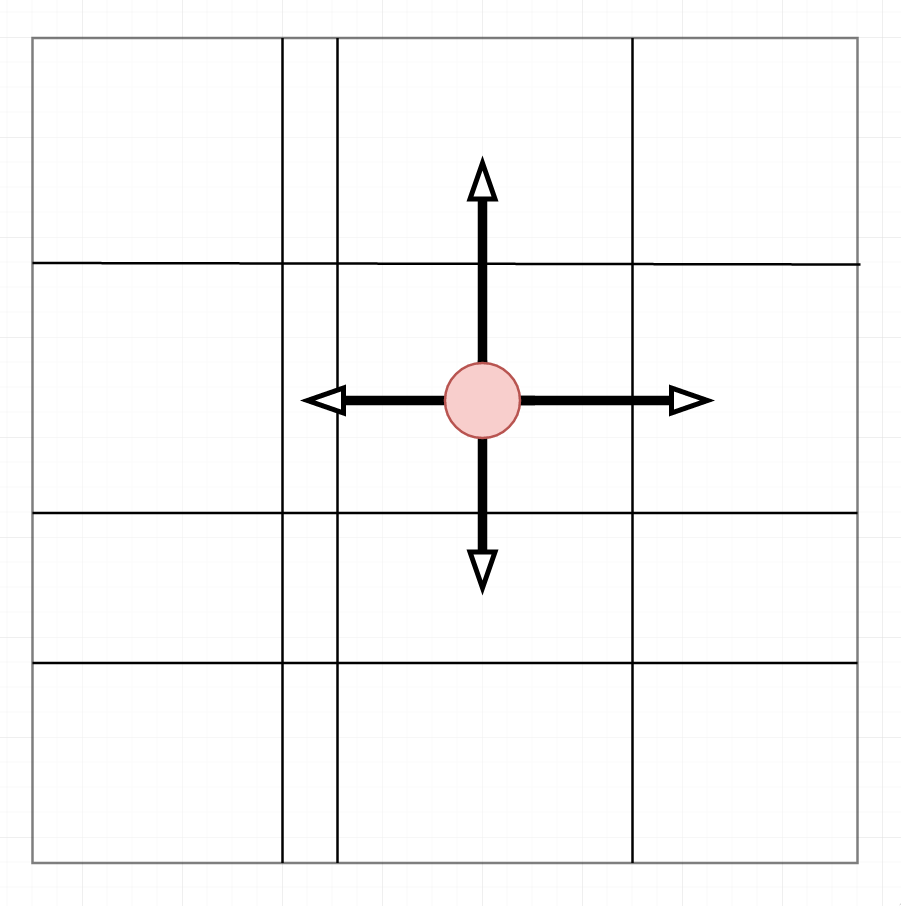
\includegraphics[width=\textwidth]{gena_move.png}
\end{columns}
\end{frame}

\begin{frame} \frametitle{Сравниваемые алгоритмы}
    \begin{itemize}
        \item Перебор
        \item Перебор с погрешностью $<5\%$
        \item Случайный
        \item Отжиг
        \item Эвристика
        \item Эвристика с погрешностью $<5\%$
        \item Эвристика с погрешностью $<15\%$
    \end{itemize}
\end{frame}

\begin{frame} \frametitle{Использованные данные}
    Использованные различные общедоступные датасеты с OpenML

    \vfill
    \begin{center}
        \begin{tabular}{|l|l|l|}

        \hline

        название        & элементы  & признаки \\

        \hline

        diabetes        & 442    & 9     \\
        boston          & 506    & 12    \\
        autoPrice       & 159    & 16    \\
        wisconsin       & 194    & 33    \\
        strikes         & 625    & 7     \\
        kin8nm          & 8192   & 9     \\
        house\_8L       & 22784  & 9     \\
        house\_16H      & 22784  & 9     \\
        mtp2            & 274    & 1143  \\

        \hline

    \end{tabular}

    \vfill
    На каждом наборе параметров проводилось 10 тестов.
    \end{center}
\end{frame}

\begin{frame} \frametitle{Тестирование (Время работы | Простой случай)}
    Небольшой датасет, <30 поддеревьев
    \vfill
    \begin{columns}
        \column{.7\textwidth}
        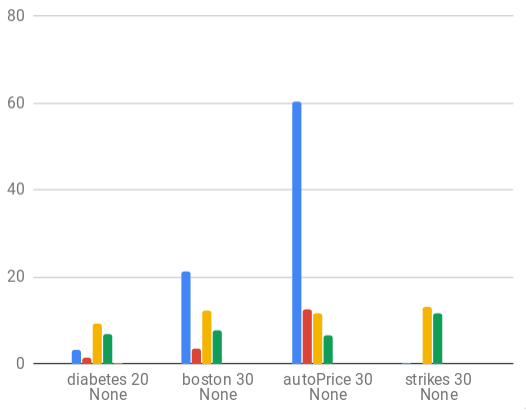
\includegraphics[width=\textwidth]{time_easy.png}
        \column{.3\textwidth}
        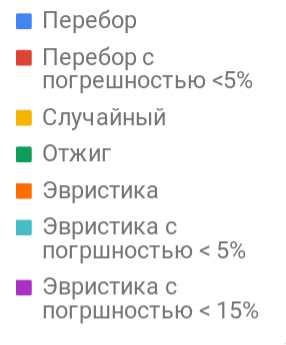
\includegraphics[width=\textwidth]{time_legend.png}
    \end{columns}
\end{frame}

\begin{frame} \frametitle{Тестирование (Время работы | Много деревьев)}
    Небольшой датасет, >30 поддеревьев
    \vfill
    \begin{columns}
        \column{.7\textwidth}
        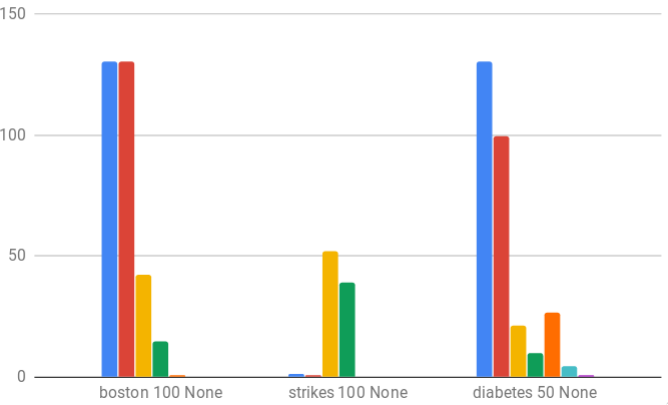
\includegraphics[width=\textwidth]{time_trees.png}
        \column{.3\textwidth}
        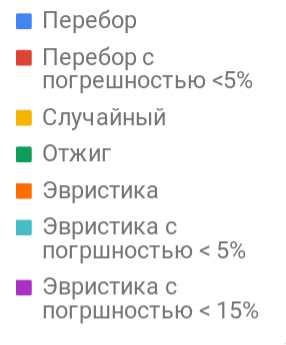
\includegraphics[width=\textwidth]{time_legend.png}
    \end{columns}
\end{frame}

\begin{frame} \frametitle{Тестирование (Время работы | Большой датасет)}
    \vfill
    \begin{columns}
        \column{.7\textwidth}
        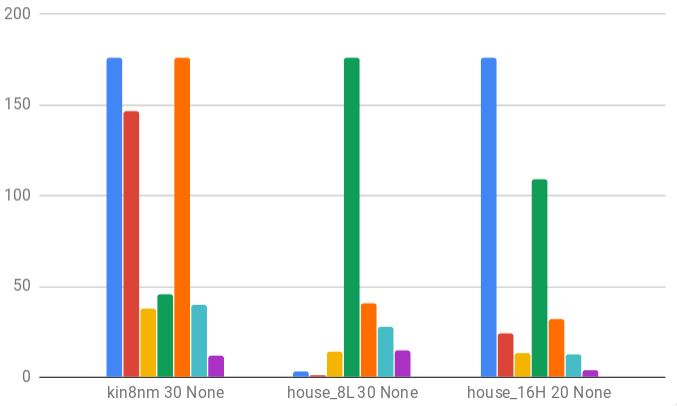
\includegraphics[width=\textwidth]{time_big.png}
        \column{.3\textwidth}
        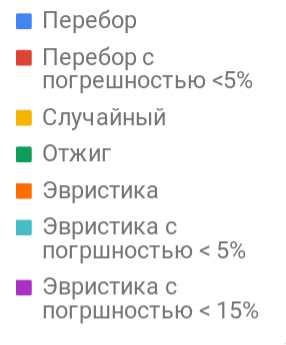
\includegraphics[width=\textwidth]{time_legend.png}
    \end{columns}
\end{frame}

\begin{frame} \frametitle{Тестирование (Ошибка | Простой случай)}
    % \[
        % error = \frac{min - min_{true} + max_{true} - max}{max_{true} - min_{true}}
    % \]
    \vfill
    \begin{columns}
        \column{.7\textwidth}
        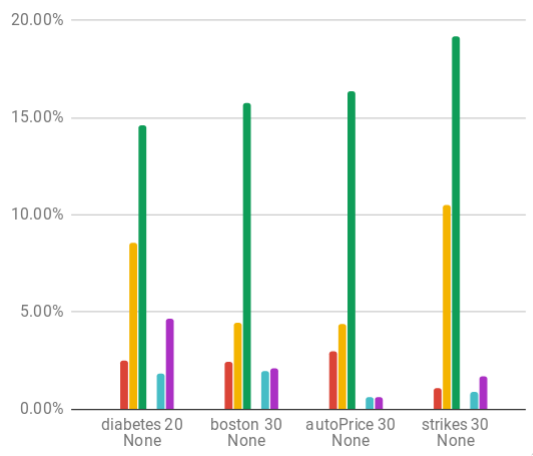
\includegraphics[width=\textwidth]{error_easy.png}
        \column{.3\textwidth}
        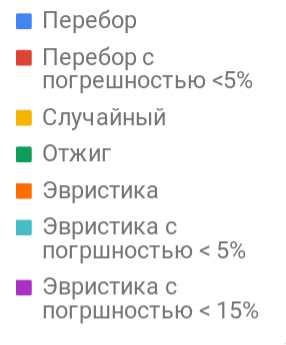
\includegraphics[width=\textwidth]{time_legend.png}
    \end{columns}
\end{frame}

\begin{frame} \frametitle{Тестирование (Ошибка | Много признаков)}
    \vfill
    \begin{columns}
        \column{.7\textwidth}
        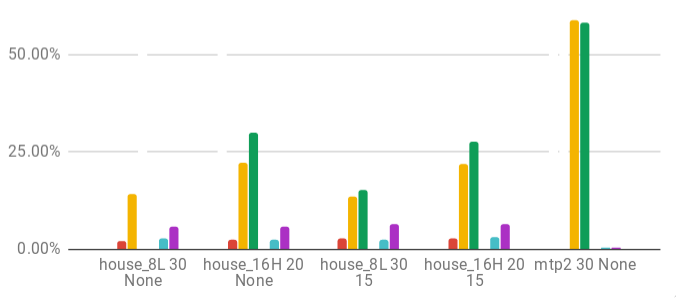
\includegraphics[width=\textwidth]{error_features.png}
        \column{.3\textwidth}
        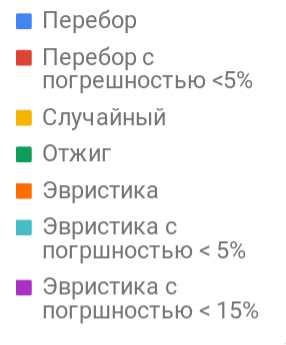
\includegraphics[width=\textwidth]{time_legend.png}
    \end{columns}
\end{frame}

\begin{frame} \frametitle{Итоги и планы}
    Отжиг
    \begin{itemize}
            \item Проблема --- переход по трешхолду из другого поддерева
            \item Решение --- хранить только трешхолды на пути до корня 
    \end{itemize}
    Эвристика
    \begin{itemize}
            \item Лучшие результаты
            \item Даже с погрешностью 15\% точность выше чем у других алгоритмов
    \end{itemize}
\end{frame}

\begin{frame} \frametitle{Тест}
    \begin{tikzpicture}
    \begin{axis}[
        enlarge x limits=0.04,
        ybar=0pt, 
        width=1.05\textwidth,
        height=0.8\textwidth,
        bar width=5pt,
        ymin=0,
        xlabel=Датасет,
        ylabel=Ошибка в \%,
        flexible xticklabels from table={../data/heuristic-15.csv}{algo}{col sep=comma},
        xticklabel style={text height=1.5ex, font=\tiny}, % To make sure the text labels are nicely aligned
        xtick=data,
    ]
    \addplot 
        [color=purple, fill=purple, fill opacity=0.33]
        plot [error bars/.cd, y dir = both, y explicit]
        table[x expr=\coordindex, y=mean_error, y error=std_error]{\random};
    \addplot 
        [color=red, fill=red, fill opacity=0.33]
        plot [error bars/.cd, y dir = both, y explicit]
        table[x expr=\coordindex, y=mean_error, y error=std_error]{\heuristicsome};
    \addplot 
        [color=blue, fill=blue, fill opacity=0.33]
        plot [error bars/.cd, y dir = both, y explicit]
        table[x expr=\coordindex, y=mean_error, y error=std_error]{\heuristicno};

    \end{axis}

    \end{tikzpicture}
\end{frame}

\end{document}
